\documentclass[border=5mm,12pt]{standalone}

\usepackage{tikz}
\usepackage{ctex}
\usetikzlibrary{calc}
\usetikzlibrary{positioning}

\tikzset{tree/.style={every node/.style={circle, draw}}}

\begin{document}

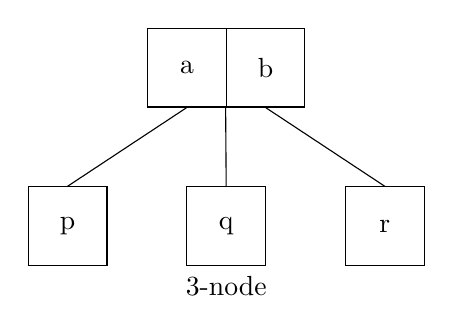
\begin{tikzpicture}[
        squarenode/.style={draw, rectangle, minimum size=1cm},
    ]
    \node[squarenode] (a) {a};
    \node[squarenode, right=-\pgflinewidth of a] (b) {b};

    \node[squarenode, below=of $(a.south)!0.5!(b.south)$] (q) {q};
    \node[squarenode, left=of q] (p) {p};
    \node[squarenode, right=of q] (r) {r};

    \draw (a.south) -- (p.north);
    \draw (b.south west) -- (q.north);
    \draw (b.south) -- (r.north);

    \node[below] at (current bounding box.south) {3-node};
\end{tikzpicture}

\end{document}
